%!TEX root = thesis.tex

%overview of the methodology to be used;

\section{Methods}
\label{chap:methods}

A number of studies related to this thesis have been reviewed in chapter \ref{chap:rw}. A discussion of the methods used in these studies (paragraph \ref{par:rwDiscuss}) resulted in a decision to adopt certain methods, such as the \ac{swe} standards, the om-lite and sam-lite ontologies, and the semantic web. This chapter will go into more detail on which methods will be used to answer the research question and how they work.  

\subsection{Sensor observation service}
There are a number of different requests that can be made to retrieve sensor (meta)data from a \ac{sos}: GetCapabilities, DescribeSensor and GetObservation. These requests can be made as a \ac{http} GET request or a \ac{http} POST request. The response is an \ac{xml} document using the \ac{om} (for GetObservation) or \ac{sensorml} (for DescribeSensor).

\subsection{Resource description framework}
For publishing static geographic data on the semantic web a conversion of Shapefiles to \ac{rdf} is required. For this the method by \cite{LD:Missier} will be used. First the Shapefile is loaded into a Postgres database with the Postgis extension. After that a Python script retrieves the records from the database. Attributes of the records will be mapped to classes from predefined ontologies. Then the script creates an \ac{rdf} graph and serialises it to a certain \ac{rdf} language. This is written it to a file. The final step is to publish the \ac{rdf} on the web and create a \ac{sparql} endpoint to query the data \citep{LD:Missier}. 

In \ac{rdf} data is stored in so-called 'triples'. These triples are structured as: subject, predicate and object \cite{LD:Berners-lee}. The subject and the object are things and the predicate is the relation between these two things. Three types of data can make up these triples. The first type is an \ac{iri}. This is a reference to a resource and can be used for all positions of the triple. A \ac{url} is an example of an \ac{iri}, but \ac{iri}s can also refer to resources without stating where a location or how it can be accessed. It is a generalisation of an \ac{uri}, also allowing non-ASCII characters. The second type of data is a literal. A literal is a value which is not an \ac{iri}, such as strings, numbers or dates. These values can only be used as object in a triple. Sometimes it's useful to refer to things without assigning them with a global identifier. The third type is the blank node and can be used as an subject or object without using an \ac{iri} or literal \citep{LD:W3C6}. 

There are a number of different notations for writing down these triples (serialisation), such as \ac{xml} \citep{LD:W3C3}, N3 \citep{LD:W3C5} and Turtle \citep{LD:W3C4}. 

The sensor metadata will also be published on the semantic web. To do this an \ac{xml} document is automatically retrieved from a \ac{sos} by a Python script. This script then extracts the relevant data from the \ac{xml} and maps it to an ontology. It outputs an \ac{rdf} file that will be published online. When new sources of sensor data are added the \ac{rdf} documents will be updated.   

\subsection{Ontology mapping}
The \ac{uml} diagram (figure \ref{fig:UML}) describes different components of a \ac{sos}. The \ac{sos} has a number of metadata attributes such as the service provider's details (including contact information), its spatial and temporal extent (spatialFiler \& temporalFilter) and the capabilities to query a subset of this extent. It receives data from a sensor which makes observations. An observation can be defined as "an action whose result is an estimate of the value of some property of the feature-of-interest, obtained using a specified procedure" \citep{SSW:Cox3}.The sensor is placed at a sampling point. The sampling point is part of a sampling feature which intents to resemble the feature-of-interest. In the case of air quality the feature-of-interest is the bubble of air surrounding the sensor, therefore the sampling point equals the feature-of-interest \citep{SDI:INSPIRE2}. The design is that an observation of the sampling feature describes the  feature-of-interest through measuring one of its properties. The measurement procedure is described by a short string of text, input and output parameters and the units of measurement of the ouput. The relation between feature-of-interest and administrative units is added to improve the discovery of sensor data on the semantic web. 

To publish data on the semantic web ontologies are required to specify the different classes and their relations. An ontology for static geographic data has to be connected to an ontology for sensor metadata. From the \ac{uml} diagram in figure \ref{fig:UML} the classes Observation, Process, ObservedProperty and FeatureOfInterest can be mapped to classes belonging to \ac{owl} for observations \citep{SSW:Cox}. SamplingFeature and Sampling point can be mapped to classes from \ac{owl} for sampling features \cite{SSW:Cox2}. GeoSPARQL can be used for the administrativeUnit class \citep{LD:OGC} and the PROV ontology for the sensor and sensor observation service classes \citep{LD:W3C2}. 

\begin{figure}
	\centering
	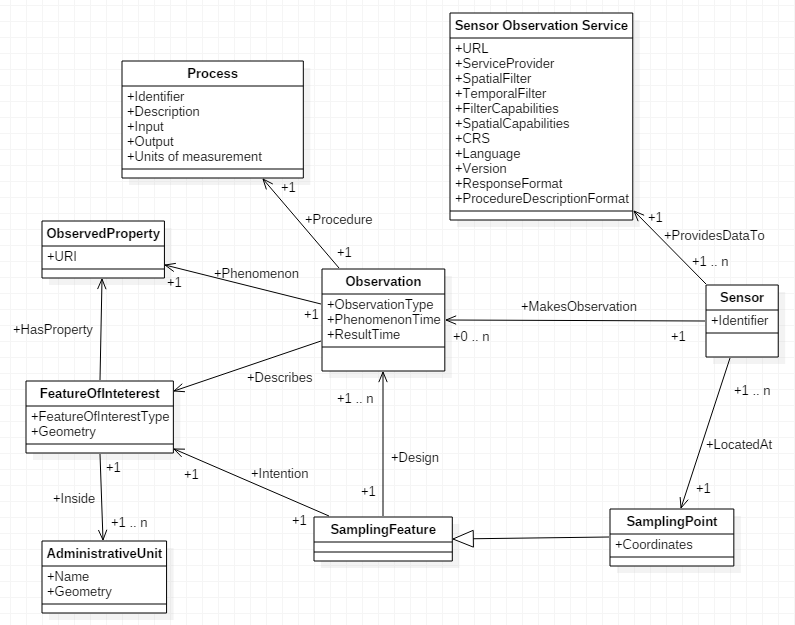
\includegraphics[width=1\linewidth]{figs/UML_Diagram.png}
	\caption{\ac{uml} diagram of sensor observations service, based on \cite{SSW:Cox3} and \cite{SDI:INSPIRE2}}
	\label{fig:UML}
\end{figure}

\subsection{Sensor data aggregation}
There are many different ways to aggregate sensor data, for example by taking the minimum value, the maximum value, the average value, the sum, etc. In order to determine which method of aggregation is applicable for a specific kind of sensor data the sensor metadata will contain links to appropriate aggregation methods. However, which methods are appropriate should be based on expert knowledge. Therefore, this requires a literature analysis. 


